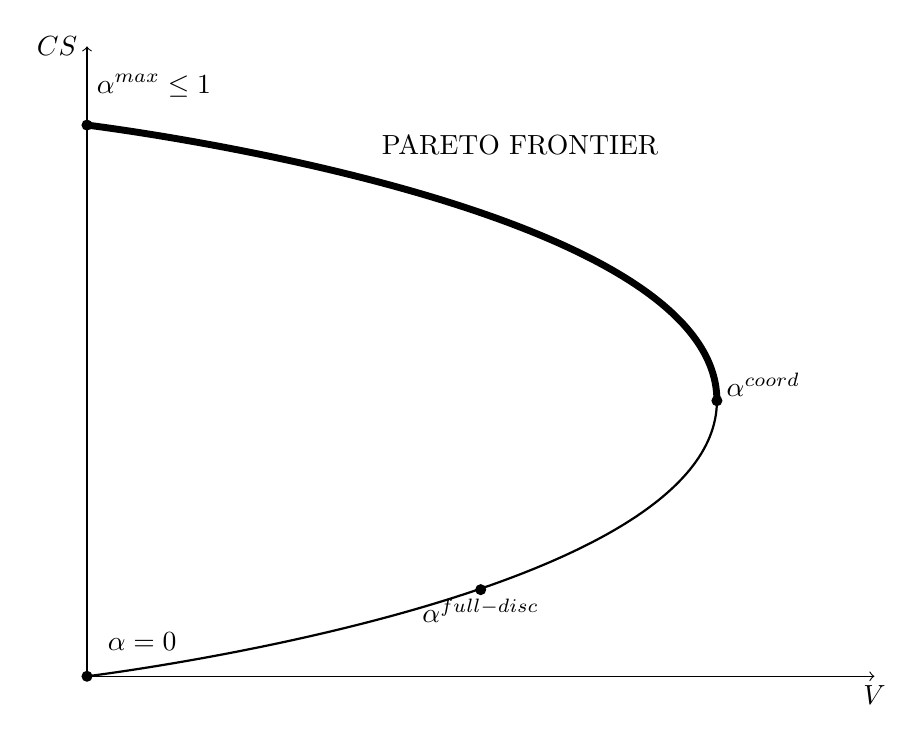
\begin{tikzpicture}[xscale=1,yscale=1] 

		\draw [<->] (0,8) node (yaxis)[left] {$CS$} 
		        |- (10,0) node (xaxis) [below] {$V$};
	\def\mycoordinates{(0,0) (8,3.5) (0,7)}

	\draw[thick,xshift=0cm] plot [smooth,tension=1.3] coordinates {\mycoordinates};
	\begin{scope}
	    \clip (0,3.5) rectangle (10,8);
	    \draw [line width=2.5] plot [smooth,tension=1.3] coordinates {\mycoordinates};
	  \end{scope}

        \fill (0,0)  circle (2pt) ;
	\node at (.7,.2)[above] {$\alpha=0$};
        \fill (8,3.5)  circle (2pt) ;
	\node at (8,3.7)[right] {$\alpha^{coord}$};
        \fill (0,7)  circle (2pt) ;
	\node at (0,7.5)[right] {$\alpha^{max}\leq 1$};
	
	\coordinate (A) at (5,1.1);
        \fill (A)  circle (2pt) ;
	\node at (A) [below] {$\alpha^{full-disc}$};


	\node at (5.5,6.5) [above] {PARETO FRONTIER};

        
\end{tikzpicture}